%--------------------------------------------------------------------------------
%----------------------------------------------------------------------
\section{The ferryman}\label{sec:ferryman}
The following is an example of a simple state-transition model sometimes used to illustrate the concept of state-transition models \cite{huth2004}. First, the model configuration is shown in the state space generation tool GROOVE. Then the same model is shown in a configuration that can be interpreted by GreenMirror. Finally, the result from the GreenMirror visualization is shown. This demonstrates the basic features, how GreenMirror can be used and how simple its usage can be. 
\par The ferryman puzzle consists of four active objects: the wolf, the goat, the cabbage and the ferryman. In the initial state of the system, the first three objects are on the left bank of a river. The ferryman is moored to the same bank with his ferry. The goal is to transport the wolf, the goat and the cabbage to the right bank of the river without the wolf eating the goat or the goat eating the cabbage. The following rules apply.
\begin{enumerate}
\item The ferryman can only bring one passenger at a time.
\item If the wolf and the goat are together on either side of the river without the ferryman present, the wolf eats the goat.
\item If the goat and the cabbage are together on either side of the river without the ferryman present, the goat eats the cabbage.
\end{enumerate}
GROOVE uses \emph{grammars} to describe the rules of a model. The grammar describing the initial state of the ferryman model is seen in \cref{fig:groove_ferryman_start}. \texttt{Wolf}, \texttt{Goat} and \texttt{Cabbage} are subtypes of the \texttt{Cargo} type. The grammars for the final states are omitted here because they are less relevant than those shown in \cref{fig:groove_ferryman_start,fig:groove_ferryman}.
\begin{figure}[h]
\centering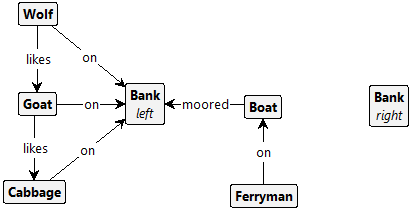
\includegraphics{images/groove_ferryman_start}
\caption{GROOVE grammar of the initial state of the ferryman model}\label{fig:groove_ferryman_start}
\end{figure}
\begin{figure}[h]
\centering
    \begin{subfigure}[b]{0.3\textwidth}
    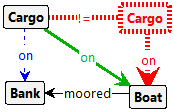
\includegraphics{images/groove_ferryman_rule_load}
    \caption{transition: load}
    \label{fig:groove_ferryman_load}
    \end{subfigure}
    ~
    \begin{subfigure}[b]{0.3\textwidth}
    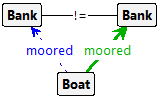
\includegraphics{images/groove_ferryman_rule_cross}
    \caption{transition: cross}
    \label{fig:groove_ferryman_cross}
    \end{subfigure}
    ~
    \begin{subfigure}[b]{0.3\textwidth}
    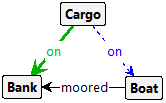
\includegraphics{images/groove_ferryman_rule_unload}
    \caption{transition: unload}
    \label{fig:groove_ferryman_unload}
    \end{subfigure}
\caption{GROOVE grammars for state-transitions of the ferryman model. The \texttt{Cargo} and \texttt{Bank} nodes are types: they indicate any cargo or river bank, respectively, that is selected with the state-transition. After the state-transition is complete, edges with a dashed blue line are removed and those with a solid green line are created. The red node and edge means: "if \texttt{Boat} has no other \texttt{Cargo} on it."}\label{fig:groove_ferryman}
\end{figure}
\par The state space generated from this model is seen in \cref{fig:groove_ferryman_statespace}. This state space contains 35 states and 70 transitions and is excellent for analysing state-transitions needed to get to a specific state. However, if one wants to visualize and animate the state-transitions that result in a specific state, these space generations tools don't have much to offer. GreenMirror can visualize this relatively easy. 
\begin{figure}[h]
	\centering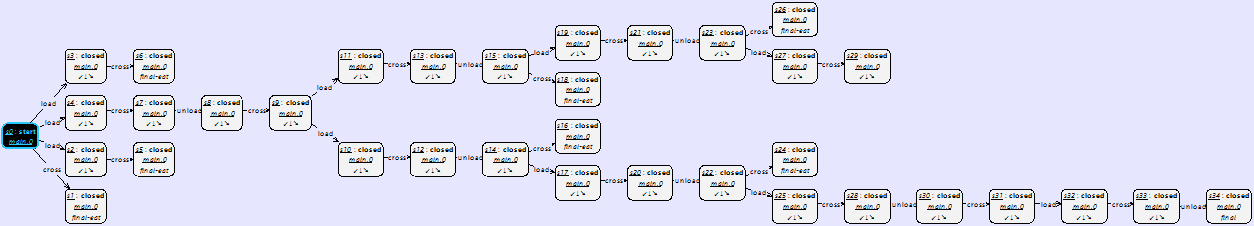
\includegraphics[width=\textwidth]{images/groove_ferryman_statespace}
    \caption{GROOVE generated state space of the ferryman model, using the breadth-first exploration strategy and final states acceptor, visualized using the compact tree layout and spanning tree filter. The blocks are the unique states and the labelled lines between them are the state-transitions. Note: because of the size of the image, the states and state-transitions are practically unreadable. This does not make the image any less relevant: it's an illustration of how a state space can become unclear easily and how it can be used to for analysis.}
    \label{fig:groove_ferryman_statespace}
\end{figure}
\par This model can be translated easily into files that can be interpreted by GreenMirror. For this example, the Groovy script model initializer and file trace selector implementations will be used (see \cref{sec:design;sub:interface}). \Cref{lst:greenmirror_ferryman_model} shows how the model is initialized. On line 1, the visualizer is initialized with a width of 500 pixels, a height of 300 pixels and a default JavaFX transition duration of 1000 milliseconds. On lines 3 to 46, the initial state is defined: the background, the ferry, the wolf, the goat and the cabbage nodes and all relations between them are created. These lines are roughly equivalent to \cref{fig:groove_ferryman_start}, with additional visualization information. Lines 49 to 58 are equivalent to \cref{fig:groove_ferryman_load}. A clear difference lies in the conditional that the ferry can not already hold a cargo node: GROOVE simply does not explore the states resulting from that state-transition, whereas GreenMirror gives an exception and aborts when this state-transition is erroneously encountered on a trace. Lines 61 to 68 and 71 to 80 are equivalent to respectively \cref{fig:groove_ferryman_cross,fig:groove_ferryman_unload}.
\lstinputlisting[label={lst:greenmirror_ferryman_model}, caption={example Groovy code for the ferryman model}]{code/ferryman.java}
\par The trace chosen for this example is the shortest trace that leads to the successful solution of the ferryman puzzle. In \cref{fig:groove_ferryman_statespace}, it is the path starting from the initial state, shown left in the figure, and ending in the state, shown in the bottom right corner of the figure. All other final states are unsuccessful solutions where either the goat or the cabbage gets eaten, or states that transition back into one of the displayed unique states. The trace is shown in \cref{lst:greenmirror_ferryman_trace}.
\lstinputlisting[label={lst:greenmirror_ferryman_trace}, caption={example trace for the ferryman model}]{code/ferryman.trace.txt}
\begin{wrapfigure}{o}{0.4\textwidth}\vspace{-22pt}
  \begin{center}
    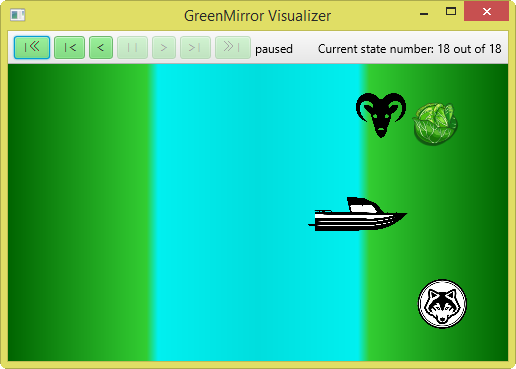
\includegraphics[width=0.38\textwidth]{images/greenmirror_ferryman}
  \end{center}
  \vspace{-10pt}\caption{a screenshot of the by GreenMirror visualized final state of the ferryman model as defined in \cref{lst:greenmirror_ferryman_model,lst:greenmirror_ferryman_trace}}\vspace{-20pt}
  \label{fig:greenmirror_ferryman}
\end{wrapfigure}
\par The ferryman model and trace from respectively \cref{lst:greenmirror_ferryman_model,lst:greenmirror_ferryman_trace} result in the GreenMirror visualization of which the final state is shown in \cref{fig:greenmirror_ferryman}. With just 80 lines of code and a pre-defined trace, the ferryman model of \cref{fig:groove_ferryman_start,fig:groove_ferryman,fig:groove_ferryman_statespace} can be visualized and animated in GreenMirror for further analysis. It took GreenMirror about one second to interpret the model and the trace, followed by roughly five seconds to add all data to the visualizer after which the user could start moving through the model states. As is seen from the code in \cref{lst:greenmirror_ferryman_model}, images, geometric shapes such as rectangles and directed relations can be used. Furthermore, nodes can be placed according to their relations and complex (programming) logic can be added. \Cref{sec:features} contains more information about the currently available features.